\textbf{Beispiel 1}\\ \\
a)\\ \\
Freigeschnittenes Fahrzeug:
\begin{figure}[h]
	\centering
	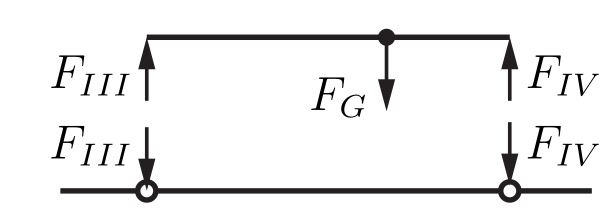
\includegraphics[width= 10cm]{tikz/28_09_2018_1a}
\end{figure}
\newline
Die Gleichgewichtsbedingungen lauten
\begin{align*}
	\textbf{e}_y &: F_{III} - F_G + F_{IV} = 0 \\
	\textbf{e}_z &: -F_{III}k + F_{IV}l = 0
\end{align*}
Aus diesen beiden Gleichungen folgen schließlich die beiden Kräfte 
\begin{align*}
	F_{III} &= \frac{l}{k + l}F_G \\
	F_{IV} &= \frac{k}{k + l}F_G
\end{align*}
b) \\ \\
Die Gleichgewichtsbedingungen mit den beiden Lagern lauten
\begin{align*}
	\textbf{e}_x &: F_{A,x} = 0\\
	\textbf{e}_y &: F_{A,y} - F_{III} - F_{IV} + F_B = 0\\
	\textbf{e}_z &: -F_{III}2a  - F_{IV}3a + F_B4a = 0
\end{align*}
Aus diesen Gleichungen folgen die Lagerkräfte
\begin{align*}
	F_{A,x} &= 0 \\
	F_{A,y} &= \frac{2l + k}{4a}F_G \\
	F_B &= \frac{2l + 3k}{4a}F_G
\end{align*}
c)\\ \\
Mit der Momentengleichung
\[
	\textbf{e}_z : -F_{A,y}2a + F_6h = 0 
\]
im Knoten III folgt die Stabkraft
\[
	F_6 = \frac{2l + k}{2h}F_G
\]
Aus diesem Ergebnis ergibt sich das der Stab 6 ein Zugstab ist. \\ \\
d)\\ \\
Durch einfaches Überlegen ergibt sich das Stab 1 ein Druck- und Stab 2 ein Zugstab ist. Die bestimmte Höhe beträgt
\[
	h = \sqrt{3}a
\]
e) \\ \\
Aus 
\begin{align*}
	\textbf{e}_x &: F_1 - F_4 = 0\\
	\textbf{e}_y &: F_3 = 0
\end{align*}
ist ersichtlich, dass auf den Stab 3 keine Kraft ausgeübt wird. \\ \\